\section{Problema 2}

\subsection{Enunciado}
En éste problema se nos pide que dada una matriz de $n$ x $m$, hallemos la cantidad de elementos de la meseta más extensa. Para ello, definimos como meseta al conjunto de celdas adyacentes sobre sus lados que comparten el mismo valor. Se nos pide, además, que resolvamos el ejercicio en, como máximo, $O((n*m)^2)$.

\subsection{Soluci\'on}
Para la resolucón de éste problema, lo que decidimos hacer fue, para cada celda de la matriz, contabilizar la cantidad de elementos que le son adyacentes y comparten su mismo valor. Para ello, recorremos recursivamente las celdas adyacentes de cada una, hasta que encontremos una cuyo valor sea diferente al que estemos analizando. Una vez encontrado dicho valor, y sabiendo la cantidad de elementos de la meseta para dicha celda, analizamos si es mayor o menos a las otras mesetas encontradas. Si es menor, la descartamos; caso contrario, guardamos la longitud de la misma hasta tanto encontremos una nueva meseta que sea mayor a la recientemente encontrada. \\
La forma que utilizamos para contar la cantidad de elementos de la meseta, como dijimos antes, es recursiva. Ésta se lleva a cabo contando, para cada celda, las posibles componentes de la meseta en una dirección de las 4 posibles (arriba, abajo, izquierda, derecha). Si en una de esas direcciones encontramos un componente de la meseta (el mismo valor de la que comenzamos) y además, esa celda no fui visitada anteriormente (es decir, no es parte de ninguna meseta ya existente), la recorremos recursivamente de la misma forma que recorrimos la celda original: para cada dirección posible, analizamos si las celdas adyacentes son parte de la meseta y de serlo, analizamos cada una de esas celdas nuevamente, de forma recursiva. Así procederemos hasta encontrar que no hay más celdas adyacentes que pertenezcan a la meseta (o, en el peor caso, que se termine nuestra matriz), y luego contaremos todas las \textit{submesetas} encontradas con el mismo valor, y que sea adyacentes, y las sumaremos entre si para calcular la cantidad de elementos de la meseta estudiada. \\
Para ir recorriendo las distintas celdas de la matriz, creamos una \textit{matriz auxiliar}, del mismo tamaño que la original, con sus valores todos en 0, y a medida que vayamos visitando las distintas celdas $i,j$ de la matriz original, iremos marcando como visitada (con un número 1) las celdas $i,j$ de la \textit{matriz auxiliar}. \\
Lo importante para mantener la complejidad lo más baja posible, y evitar visitar varias veces la misma celda, está en utilzar nuestra \textit{matriz auxiliar} para saber si ya pasamos o no por dicha celda, y no vistarla nuevamente. La razón por la que podemos hacer ésto es que si ya visité dich celda en otra ocasión, entonces no puede pertenecer a la meseta que estoy estudiando en éste momento y, por tanto, no debo considerala.

\subsection{Pseudoc\'odigo}

\begin{codebox}
\Procname{$\proc{Resolver}$ (\textbf{in} $matriz$)}{mesetaMaxima}{Int}
\li	arrayAux = CrearArrayAux(arrOrig)
\li	\textbf{Para} cada celda de la matriz \textbf{Hacer:} \Do
\li	mesetaMaximaCelda = $Contar$(celda)
\li	\textbf{Si} mesetaMaximaCelda es mayor a la mesetaMaxima actual \textbf{Hacer:} \Do
\li	Reemplazo el valor de mesetaMaxima por el de mesetaMaximaCelda
\End
\End
\li	devuelvo el valor de la mesetaMaxima
\end{codebox}

\begin{codebox}
\Procname{$\proc{Contar}$ ($celda$)}{meseta maxima de la celda}{Int}
\li	largo de la meseta = 1
\li	\textbf{Para} cada una de las celdas adyacentes \textbf{Hacer:} \Do 
\li	sumo al largo de la meseta el tamaño de la meseta de la celda adyacente
\End
\li	devuelvo el largo de la meseta
\end{codebox}

\subsection{Analisís de complejidad}	
En éste ejercicio, podríamos mencionar como 3 las partes importantes que afectan a la complejidad del mismo: la creacion de la matriz leyendo del archivo de entrada, la creación de una matriz auxiliar y el "recorrido" recursivo de la matriz para ir sabiendo la cantidad de elementos pertenecientes a una meseta tiene cada celda.
El enunciado nos pedía que, como máximo, la complejidad del algoritmo debía ser de $O((n * m)^2)$ y, de acuerdo a nuestro cálculos, nuestro algoritmo baja dicha complejidad notoriamente, ya que realiza todos los pasos (y para todos los casos, como veremos en la parte de Test y Gráficos) en $k(n * m)$, donde $k \approx 3$. \\
Decimos que k es $"$aproximadamente 3$"$ ya que no estamos contabilizando, por ejemplo, la complejidad de crear un ArrayList o de agrandarlo una vez que todos sus elementos están llenos, pero éstos se tornan casi despreciables a partir de valores de m y n relativamente pequeños. \\
Por otro lado, como dijimos, las 3 pasos más importantes del ejercicio, se realizan en la misma cantidad de ciclos, ya que en todos ellos, lo más importante que tiene que hacer el algoritmos es recorrer celda por celda una matriz (fila a fila). Cómo sabemos, la complejidad de recorrer una matriz depende del tamaño de la matriz ( n x m ), y por tanto podemos decir que la complejidad del ejercicio es $O(m*n)$, ya que el 3 es despreciable para entradas muy grandes. \\
Por último, y con respecto a por qué nuestro algoritmos de $Contar$, a pesar de ser recursivo, es considerado lineal, se debe a que nuestra implementación hace uso de una matriz auxiliar que, si bien crearla es igual de costosa que recorrer toda la matriz una vez, a la larga nos ahorra visitar celdas que ya fueron visitadas y no debería volverse a analizar. Esto es posible ya que el enunciado nos dice que sólo debemos contabilizar los valores iguales que estén en mesetas adyacentes y, por tanto, si ya visitamos una celda adyacente a la que estamos analizando, se debe únicamente a dos situaciones: o bien, ya la contabilizamos en nuestra meseta actual, o bien, ya fue visitada mientras contabilizabamos otra meseta. Cualquiera sea la situación, es claro que en ninguna de las dos deberíamos contabilizar la celda. Por tanto, podemos decir que, a pesar de ser recursivo, nuestro algoritmos, ayudado de su \textit{matrix auxiliar}, se comporta de manera linear. \\

\subsection{Tests y Gráficos}

En ésta seccion mostraremos los resultados de nuestras pruebas que utilizamos para comprobar que, en todos los casos posibles, el ejercicio actúa siempre de la misma forma. \\
Los casos que tuvimos en cuenta fueron 3: aquellos donde los valores de la matriz son todos distintos (y, por tanto, la meseta máxima sería 1), aquellos donde son todos iguales (donde habría una sola meseta, la matriz entera, y su valor sería el de $m x n$) y, por último, aquellos en que los valores son aleatorios (y de donde no podemos inferir nada acerca del tamaño de la matriz). \\
Todos los casos los analizamos contra la misma variable: cantidad de ciclos realizados por nuestro ejercicio. Para ello, generamos valores de entradas que cumplieran dichas pautas (que los valores de las celdas sean iguales, distintos o aleatorios), y con valores de n y m variables.  \\

\begin {center}
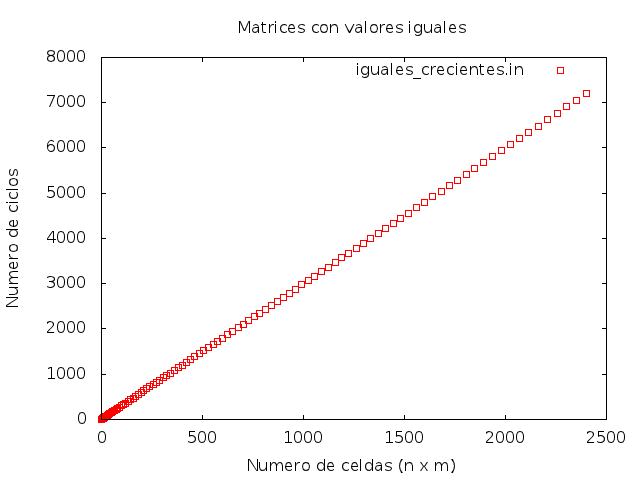
\includegraphics[width=8cm]{./graficos/igualesCrecientes.png}
% grafico.eps: 0x0 pixel, 300dpi, 0.00x0.00 cm, bb=50 50 410 302
\end {center} 

\begin {center}
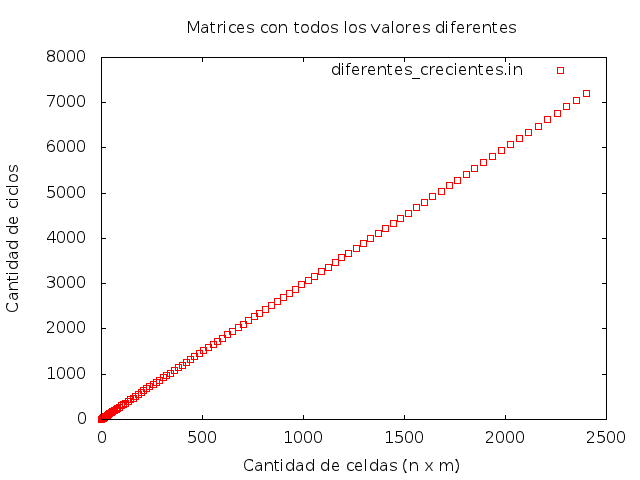
\includegraphics[width=8cm]{./graficos/diferentesCrecientes.png}
% grafico.eps: 0x0 pixel, 300dpi, 0.00x0.00 cm, bb=50 50 410 302
\end {center} 

\begin {center}
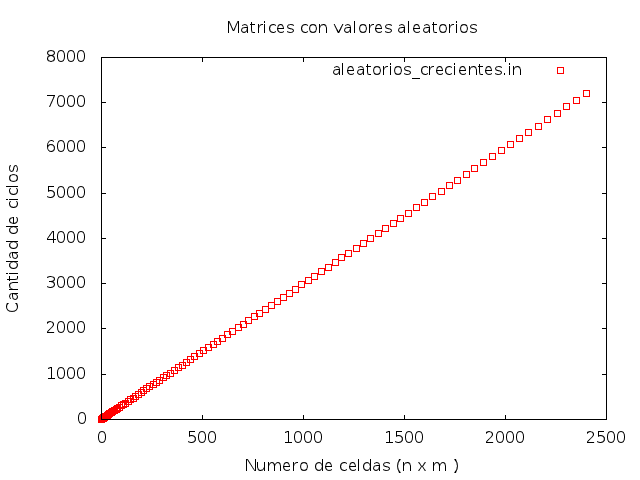
\includegraphics[width=8cm]{./graficos/aleatoriosCrecientes.png}
% grafico.eps: 0x0 pixel, 300dpi, 0.00x0.00 cm, bb=50 50 410 302
\end {center}

Como se puede apreciar en los tres gráficos, el resultado de los test está mostrando claramente que la complejidad de los algoritmos es totalmente independiente de cómo recibimos la entrada (ordenada, desorneda, totalmente aleatoria), sino más bien que es linealmente dependiente de el tamaño de la entrada, en éste caso, n y m. \\

\subsection{Conclusiones}
Como pudimos ver en nuestro análisis y en los test, se puede decir que el ejercico desarrollado es muy eficiente, ya que tarda menos de lo que nos pide el enunciado y, en particular, menos de lo que tardaría con otras técnicas algorítmicas (como lo es Programación Dinámica, que en su momento se pensó en utilizarla para resolver éste ejercicio). Por ejemplo, si hubieramos desarrollado con PD, iríamos visitando celda por celda, y para cada celda debería calcular el valor de todas las submesetas existentes, y luego ir sumandolas. De todas formas, hay celdas que contaríamos o visitaríamos más de una vez, y si bien la complejidad no sería mucho peor a la que estamos manejando en nuestra solución, se visitarían más celdas de las necesarias con nuestra implementación. \\
